\vspace{0.5cm} 

This chapter focuses on the material covered in \textit{OI Biostat} Chapter 2, which focuses on the idea of probability and how to solve for various types of probabilities. This chapter will work through several examples, illustrating how \textsf{R} can be used to solve propability problems.  Once again, it will be shown that there are several different computational methods that can be used to answer the same question.  

\section{Simple Probability}
\subsection{Through Simulation}
A powerful method for calculating probabilities in \textsf{R} is called \textbf{simulation} and consists of simulating a large population with some consistent known parameters so that population statistics can be measured.  For example, simulation can be used to obtain the probability distribution of the sum of two dice seen in \textit{OI Biostat} Figure 2.7.  

The steps for a simulation process are as follows, 
\begin{enumerate}
  \item Define the parameters of the simulation: population size.
  
  \item In order for the results of the simulation to be reproducible, it is necessary to use \texttt{set.seed()} to associate the particular set of results with a "seed". Any integer can be used as the seed. Different seeds will produce a different set of results. 
  
  \item Using the \texttt{vector()} command, create one empty list that will be used to store the results of the simulation.  
  
  \item Simulate rolling each of the dice using the  \texttt{sample()} command, which takes a sample of a specified size from a list \texttt{x}. In this context, the goal is to sample the integers between \texttt{1} and \texttt{6} 100,000 times, where the result represents the face of the die that shows up.  This is done in combination with a \texttt{for} loop.  The loop allows for this process to be repeated for each of the 100,000 individuals being simulated.  The first line sets up the loop, with a variable \texttt{ii} that starts at \texttt{1} and finishes at \texttt{population.size}, which was specified earlier as 100,000. This allows for each dice roll to be performed one at a time.
  
  \item Look at your final results of the simulated population distribution, and if desired, calculate population statistics. 

\end{enumerate}


\begin{knitrout}
\definecolor{shadecolor}{rgb}{0.969, 0.969, 0.969}\color{fgcolor}\begin{kframe}
\begin{alltt}
\hlcom{## 1. Set parameters}
\hlstd{population.size} \hlkwb{=} \hlnum{1e+05}

\hlcom{## 2. Set Seed}
\hlkwd{set.seed}\hlstd{(}\hlnum{2016}\hlstd{)}

\hlcom{## 3. Create empty list}
\hlstd{dice.sums} \hlkwb{=} \hlkwd{vector}\hlstd{(}\hlstr{"numeric"}\hlstd{, population.size)}

\hlcom{## 4. Simulate 'rolling the dice'}
\hlkwa{for} \hlstd{(ii} \hlkwa{in} \hlnum{1}\hlopt{:}\hlstd{population.size) \{}
    \hlstd{dice.1} \hlkwb{=} \hlkwd{sample}\hlstd{(}\hlnum{1}\hlopt{:}\hlnum{6}\hlstd{,} \hlkwc{size} \hlstd{=} \hlnum{1}\hlstd{)}
    \hlstd{dice.2} \hlkwb{=} \hlkwd{sample}\hlstd{(}\hlnum{1}\hlopt{:}\hlnum{6}\hlstd{,} \hlkwc{size} \hlstd{=} \hlnum{1}\hlstd{)}
    \hlstd{dice.sums[ii]} \hlkwb{=} \hlstd{dice.1} \hlopt{+} \hlstd{dice.2}
\hlstd{\}}

\hlcom{## 5. Plot results}
\hlkwd{hist}\hlstd{(dice.sums,} \hlkwc{freq} \hlstd{=} \hlnum{FALSE}\hlstd{,} \hlkwc{ylab} \hlstd{=} \hlstr{"Probability"}\hlstd{,} \hlkwc{xlab} \hlstd{=} \hlstr{"Dice Sum"}\hlstd{,} \hlkwc{main} \hlstd{=} \hlstr{""}\hlstd{)}
\end{alltt}
\end{kframe}

{\centering 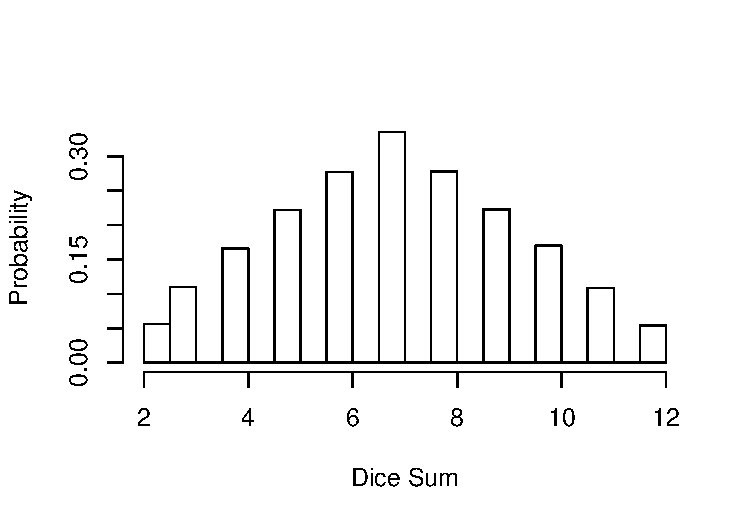
\includegraphics[width=\maxwidth]{figure/unnamed-chunk-1-1} 

}



\end{knitrout}


\section{Conditional Probability}
What are the chances that a woman with a positive mamogram has breast cancer? This question can be rephrased as the conditional probability that a woman has breast cancer, given that her mammogram is abnormal, otherwise known as the \textbf{positive predictive value} of a mammogram. Two methods discussed in this chapter, using Bayes' Theorem and creating a contingency table, are also explained in \textit{OI Biostat}. This chapter will also cover an additional approach: modeling the problem scenario by running a simulation.

\begin{quotation}

\textbf{\textit{OI Biostat} Example 2.37.} In Canada, about 0.35\% of women over 40 will develop breast cancer in any given year. A common screening test for cancer is the mammogram, but it is not perfect. In about 11\% of patients with breast cancer, the test gives a \textbf{false negative}: it indicates a woman does not have breast cancer when she does have breast cancer. Similarly, the test gives a \textbf{false positive} in 7\% of patients who do not have breast cancer: it indicates these patients have breast cancer when they actually do not. If a randomly selected woman over 40 is tested for breast cancer using a mammogram and the test is positive -- that is, the test suggests the woman has cancer -- what is the probability she has breast cancer?

\end{quotation}

\subsection{Bayes' Theorem}

Bayes' Theorem states that the conditional probability $P(A_1 | B)$ can be identified as the following fraction:\vspace{-1.5mm}
\begin{align*}
\frac{P(A_1 \text{and } B)}{P(B)}= \frac{P(B | A_1) P(A_1)}
	{P(B | A_1) P(A_1) + P(B | A_2) P(A_2) + \cdots + P(B | A_k) P(A_k)}
\end{align*}
where $A_2$, $A_3$, ..., and $A_k$ represent all other possible outcomes of the first variable.

The expression can also be written in terms of diagnostic testing language, where $D = \text{\{has disease\}}$, $D^c = \text{\{does not have disease\}}$, $T^{+} = \text{\{positive test result\}}$, and $T^{-} = \text{\{negative test result\}}$.

\begin{align*}
P(D|T^{+}) &= \dfrac{P(D \text{ and } T^{+})}{P(D)} \\
&= \dfrac{P(T^{+}|D) \times P(D)}{[P(T^{+}|D) \times P(D)] + [P(T^{+}|D^c) \times P(D^c)]} \\
\text{PPV} &= \dfrac{\text{sensitivity } \times \text{ prevalence}}{[\text{sensitivity } \times \text{ prevalence}] + [\text{(1 - specificity) } \times \text{ (1 - prevalence)}]}
\end{align*}

\textsf{R} can be used to store values for prevalence, sensitivity, and specificity so that calculations are less tedious. Recall that the \textbf{sensitivity} is the probability of a positive test result when disease is present, which is the complement of a false negative. The \textbf{specificity} is the probability of a negative test result when disease is absent, which is the complement of a false positive.  With this in mind, solving for the \textbf{positive predictive value (PPV)} is quite easy in \textsf{R} for the breast cancer example as follows.  

\begin{knitrout}
\definecolor{shadecolor}{rgb}{0.969, 0.969, 0.969}\color{fgcolor}\begin{kframe}
\begin{alltt}
\hlstd{prevalence} \hlkwb{=} \hlnum{0.0035}
\hlstd{sensitivity} \hlkwb{=} \hlnum{1} \hlopt{-} \hlnum{0.11}
\hlstd{specificity} \hlkwb{=} \hlnum{1} \hlopt{-} \hlnum{0.07}

\hlstd{ppv.num} \hlkwb{=} \hlstd{(sensitivity}\hlopt{*}\hlstd{prevalence)}  \hlcom{## numerator}
\hlstd{ppv.den} \hlkwb{=} \hlstd{ppv.num} \hlopt{+} \hlstd{((}\hlnum{1}\hlopt{-}\hlstd{specificity)}\hlopt{*}\hlstd{(}\hlnum{1}\hlopt{-}\hlstd{prevalence))}  \hlcom{## denominator}
\hlstd{ppv} \hlkwb{=} \hlstd{ppv.num} \hlopt{/} \hlstd{ppv.den}

\hlstd{ppv}
\end{alltt}
\begin{verbatim}
## [1] 0.04274736
\end{verbatim}
\end{kframe}
\end{knitrout}


\subsection{Contingency Table}

The PPV can also be calculated by constructing a two-way contingency table for a hypothetical population and calculating conditional probabilities by conditioning on rows or columns. While this method results in an estimate of PPV, using a large enough population size such as 100,000 produces an empirical estimate that is very close to the exact value found through using Bayes' Theorem. 

\begin{center}
\begin{tabular}{|l|c|c|r|}
\hline 
& D+ & D- & Total\\ 
\hline
T+ & & & \\ 
\hline
T- & & & \\ 
\hline 
Total & & & 100,000 \\ 
\hline 
\end{tabular} 
\end{center} 

First, calculate the expected number of disease cases and non-disease cases in the population:
\begin{knitrout}
\definecolor{shadecolor}{rgb}{0.969, 0.969, 0.969}\color{fgcolor}\begin{kframe}
\begin{alltt}
\hlstd{population.size} \hlkwb{=} \hlnum{100000}
\hlstd{expected.cases} \hlkwb{=} \hlstd{prevalence} \hlopt{*} \hlstd{population.size}
\hlstd{expected.cases}
\end{alltt}
\begin{verbatim}
## [1] 350
\end{verbatim}
\begin{alltt}
\hlstd{expected.noncases} \hlkwb{=} \hlstd{(}\hlnum{1} \hlopt{-} \hlstd{prevalence)} \hlopt{*} \hlstd{population.size}
\hlstd{expected.noncases}
\end{alltt}
\begin{verbatim}
## [1] 99650
\end{verbatim}
\end{kframe}
\end{knitrout}

\begin{center}
\begin{tabular}{|l|c|c|r|}
\hline 
& D+ & D- & Total\\ 
\hline
T+ & & & \\ 
\hline
T- & & & \\ 
\hline 
Total & 350 & 99,650 & 100,000 \\ 
\hline 
\end{tabular} 
\end{center}

Next, calculate the expected number of cases of true positives and the expected number of cases of false positives:  
\begin{knitrout}
\definecolor{shadecolor}{rgb}{0.969, 0.969, 0.969}\color{fgcolor}\begin{kframe}
\begin{alltt}
\hlstd{expected.true.positives} \hlkwb{=} \hlstd{expected.cases} \hlopt{*} \hlstd{sensitivity}
\hlstd{expected.true.positives}
\end{alltt}
\begin{verbatim}
## [1] 311.5
\end{verbatim}
\begin{alltt}
\hlstd{expected.false.positives} \hlkwb{=} \hlstd{expected.noncases} \hlopt{*} \hlstd{(}\hlnum{1} \hlopt{-} \hlstd{specificity)}
\hlstd{expected.false.positives}
\end{alltt}
\begin{verbatim}
## [1] 6975.5
\end{verbatim}
\begin{alltt}
\hlstd{total.expected.positives} \hlkwb{=} \hlstd{expected.true.positives} \hlopt{+} \hlstd{expected.false.positives}
\hlstd{total.expected.positives}
\end{alltt}
\begin{verbatim}
## [1] 7287
\end{verbatim}
\end{kframe}
\end{knitrout}

 
\begin{center}
\begin{tabular}{|l|c|c|r|}
\hline 
& D+ & D- & Total\\ 
\hline
T+ & 311.5 & 6,975.5 & 7,287\\ 
\hline
T- & & & \\ 
\hline 
Total & 350 & 99,650 & 100,000 \\ 
\hline 
\end{tabular} 
\end{center}

Finally, calculate the positive predictive value: 
\begin{knitrout}
\definecolor{shadecolor}{rgb}{0.969, 0.969, 0.969}\color{fgcolor}\begin{kframe}
\begin{alltt}
\hlstd{ppv} \hlkwb{=} \hlstd{expected.true.positives}\hlopt{/}\hlstd{total.expected.positives}
\hlstd{ppv}
\end{alltt}
\begin{verbatim}
## [1] 0.04274736
\end{verbatim}
\end{kframe}
\end{knitrout}


\subsection{Simulation}

% JV: will definitely be good to have some simple simulation exercises for this chapter, like the drug testing example from 102

The final method for solving this conditional probability problem in \textsf{R} is through \textbf{simulation} and involves the process of simulating 100,000 individuals who each have the same probability of having the disease.  Afterwards, using the known specificity and sensitivity of the diagnostic test, individuals can be assigned a test result of either positve or negative as if a test had been performed.  This results in a simulated dataset of 100,000 individuals that each have a disease status and test result. 

\begin{enumerate}
  \item Define the parameters of the simulation: disease prevalence, test sensitivity, test specificity, and hypothetical population size.
  
  \item In order for the results of the simulation to be reproducible, it is necessary to use \texttt{set.seed()} to associate the particular set of results with a "seed". Any integer can be used as the seed. Different seeds will produce a different set of results. 
  
  \item Using the \texttt{vector()} command, create two empty lists that will be used to store the results of the simulation: one will store disease status and the other will store test outcome. The results will be in the form of numbers; specifically, either \texttt{0} or \texttt{1}. 
  
  \item Assign disease status by using the \texttt{sample()} command, which takes a sample of a specified size from a list \texttt{x}. In this context, the goal is to sample between \texttt{0} and \texttt{1} 100,000 times, where \texttt{0} represents an individual without breast cancer and \texttt{1} an individual with breast cancer. The argument \texttt{prob} defines the probability that either number is sampled; a \texttt{1} should be sampled with the same probability as the prevalence, since the prevalence indicates how many members of the population have disease. Similarly, a \texttt{0} should be sampled with probability \texttt{(1 - prevalence)}. The argument \texttt{replace = TRUE} allows for sampling with replacement; in other words, allowing the numbers \texttt{0} and \texttt{1} to be assigned multiple times. 
  
  \item Assign test result by using the \texttt{sample()} command in combination with a \texttt{for} loop and conditional statements. In this step, a test result is assigned with different probability depending on whether the disease status is a \texttt{0} or a \texttt{1}; this relates to the sensitivity and specificity of the diagnostic test. The loop allows for this process to be repeated for each of the 100,000 individuals being simulated.
  
  \begin{itemize}
    \item The first line sets up the loop, with a variable \texttt{ii} that starts at \texttt{1} and finishes at \texttt{population.size}, which was specified earlier as 100,000. This allows for each test result to be assigned one at a time.
    
    \item Two \texttt{if} statements are in the loop which direct \textsf{R} to take a different action depending on the value of \texttt{disease.status}. The double equals signs \texttt{==} imply a conditional statement, allowing \texttt{if(disease.status[ii] == 1)} to make the statement "For this loop, if disease status is equal to 1, then do the following...".
    
    \item Depending on disease status, \textsf{R} will execute one of the two \texttt{sample()} functions in the loop. One sample function has probabilities weighted based on sensitivity and the other has probabilities defined by specificity. 
  
  \end{itemize}
  
  \item Make calculations using the two lists, \texttt{disease.status} and \texttt{disease.outcome}, which are now filled with values. Since the value \texttt{1} was assigned to a positive test result and to an individual with disease, the \texttt{sum()} command can be used to determine the total number of individuals with disease and the number of positive test results. 

\end{enumerate}


\begin{knitrout}
\definecolor{shadecolor}{rgb}{0.969, 0.969, 0.969}\color{fgcolor}\begin{kframe}
\begin{alltt}
\hlcom{## 1. set parameters}
\hlstd{prevalence} \hlkwb{=} \hlnum{0.0035}
\hlstd{sensitivity} \hlkwb{=} \hlnum{1} \hlopt{-} \hlnum{0.11}
\hlstd{specificity} \hlkwb{=} \hlnum{1} \hlopt{-} \hlnum{0.07}
\hlstd{population.size} \hlkwb{=} \hlnum{100000}

\hlcom{## 2. set seed}
\hlkwd{set.seed}\hlstd{(}\hlnum{2016}\hlstd{)}

\hlcom{## 3. create empty lists}
\hlstd{disease.status} \hlkwb{=} \hlkwd{vector}\hlstd{(}\hlstr{"numeric"}\hlstd{, population.size)}
\hlstd{test.outcome} \hlkwb{=} \hlkwd{vector}\hlstd{(}\hlstr{"numeric"}\hlstd{, population.size)}

\hlcom{## 4. assign disease status}
\hlstd{disease.status} \hlkwb{=} \hlkwd{sample}\hlstd{(}\hlkwc{x} \hlstd{=} \hlkwd{c}\hlstd{(}\hlnum{0}\hlstd{,}\hlnum{1}\hlstd{),} \hlkwc{size} \hlstd{= population.size,}
                        \hlkwc{prob} \hlstd{=} \hlkwd{c}\hlstd{(}\hlnum{1} \hlopt{-} \hlstd{prevalence, prevalence),}  \hlcom{## matches order of x}
                        \hlkwc{replace} \hlstd{=} \hlnum{TRUE}\hlstd{)}

\hlcom{## 5. assign test result}
\hlkwa{for} \hlstd{(ii} \hlkwa{in} \hlnum{1}\hlopt{:}\hlstd{population.size) \{}
  \hlkwa{if} \hlstd{(disease.status[ii]} \hlopt{==} \hlnum{1}\hlstd{) \{}  \hlcom{## note the ==}
    \hlstd{test.outcome[ii]} \hlkwb{=} \hlkwd{sample}\hlstd{(}\hlkwd{c}\hlstd{(}\hlnum{0}\hlstd{,} \hlnum{1}\hlstd{),} \hlkwc{size} \hlstd{=} \hlnum{1}\hlstd{,} \hlcom{## test results assigned 1 at a time}
                              \hlkwc{prob} \hlstd{=} \hlkwd{c}\hlstd{(}\hlnum{1} \hlopt{-} \hlstd{sensitivity, sensitivity))\}}
  \hlkwa{if} \hlstd{(disease.status[ii]} \hlopt{==} \hlnum{0}\hlstd{) \{}  \hlcom{## note the ==}
    \hlstd{test.outcome[ii]} \hlkwb{=} \hlkwd{sample}\hlstd{(}\hlkwd{c}\hlstd{(}\hlnum{0}\hlstd{,} \hlnum{1}\hlstd{),} \hlkwc{size} \hlstd{=} \hlnum{1}\hlstd{,} \hlcom{## test results assigned 1 at a time}
                              \hlkwc{prob} \hlstd{=} \hlkwd{c}\hlstd{(specificity,} \hlnum{1} \hlopt{-} \hlstd{specificity))\}}

\hlstd{\}}

\hlcom{## 6. calculate ppv}
\hlstd{num.disease} \hlkwb{=} \hlkwd{sum}\hlstd{(disease.status)}  \hlcom{## total number of individuals with disease}
\hlstd{num.pos.test} \hlkwb{=} \hlkwd{sum}\hlstd{(test.outcome)}   \hlcom{## total number of positive tests}

\hlcom{# identify the number of individuals with disease who tested positive}
\hlstd{num.true.pos} \hlkwb{=} \hlkwd{sum}\hlstd{(test.outcome[disease.status} \hlopt{==} \hlnum{1}\hlstd{])}

\hlcom{# calculate ppv}
\hlstd{ppv} \hlkwb{=} \hlstd{num.true.pos} \hlopt{/} \hlstd{num.pos.test}
\hlstd{ppv}
\end{alltt}
\begin{verbatim}
## [1] 0.04273973
\end{verbatim}
\end{kframe}
\end{knitrout}



%

%The first step in this process is to set some defined parameters as follows.  Note that the last line "sets a seed" for our simulation.  To perform the simulation, we will be using random number generation, and this line guarantees that we are getting the same set of "random" numbers everytime we perform the simulation.  It does not affect the results at all, but rather is just to compare work between colleagues or compare against a previous simulation. Any integer can be put into the seed command.   
%<<>>=
%#parameters
%prevalence = 1/6000 
%sensitivity = 0.950 
%specificity = 0.99897
%population.size = 100000
%set.seed(8)
%@

%Next, we must create a space where we can store the information about our simulated individuals.  Imagine as if you wrote on a sheet of paper the numbers 1 through 100,000 and left a blank line next to each number.  You could then go back and fill in each line with the information you wanted to.  We can create two empty lists as follows, one for the patient disease status and one for their test outcomes.  
%<<>>=
%disease.presence = vector("numeric", population.size)
%test.outcome = vector("numeric", population.size)
%@

%Next, we must determine whether each individual in our simulated population has the disease or not.  We know the prevalence of the disease, so for each individual we can say that $P(D+) = prevalence$.  For the data storage, we will keep track of diseased individuals as 1 and non-diseased individuals as 0.  The following line determines the disease status by either giving outcomes of 0 or 1, as indicated by the command $x = c(0,1)$. The next element of size dictates how many individuals the $sample$ should consider, in this case 100,000 individuals.  Next, we dictate the probability of each outcome in our list of possible outcomes $x$.  This prob element must have the same number of possibilities as $x$ and each element corresponds to the same element in $x$.  We see that for each individual, the probability of no disease, or 0, will be $1-prevalence$ and the probability of disease, or 1, will be $prevalence$.  The last element of this command is "replace = TRUE", and this commands tells the computer whether or not to return a possible outcome to the selection options after it has been picked once.  For example, if the first person has no disease, i.e. they have outcome 0, this command says to put the 0 back in the options list, $x$, for the next person to possibly have.  Essentially, this just means that values in $x$ can be repeated.  
%<<>>=
%disease.status = sample(x = c(0,1), size = population.size, prob=c(1 - prevalence, 
%              prevalence), replace = TRUE)
%@

%Next, we perform our simulation using a process called \textbf{looping}.  Looping is the idea that we want to perform the same set of steps for each individual.  This set of steps includes looking at the disease status for each individual and if they are diseased, considering the sensitivity to determine their test result, or if they are not diseased, considering the specificity to determine their test result.  This point illustrates a key idea of why we use simulation studies.  In a real life study, when a test is performed, the true disease status is not actually known, which is why you are performing the test.  However, in this case, we can simulate true disease status as if we were omnipotent, and then, see how the test would react based on that.

%There are a lot of commands in here, so let's try to break them down a bit.  The first one we see is our loop, the command $for$.  This command simply takes the numbers 1 through 100,000 as dictated by the code "1:population.size" and scrolls through them one at a time.  It starts by setting a variable $ii$ equal to 1, then all of the code inside the brackets is executed, then it sets $ii$ equal to the next number and so forth.  Within this loop are two $if$ statements, which operate by checking if the code inside the parentheses is true and if so, performing the code inside the brackets.  If not, the code inside the brackets is skipped over.  In this case, we see the code inside the $if$ parentheses says $disease.status[ii] ==1$, and this is testing whether or not the disease status of the $ii$th person is equal equal to 1.  The two equals signs here imply the question of whether or not the left hand side is equal to the right hand side.  The next $if$ statement does the opposite by testing whether or not an individual is not diseased, i.e. having disease status of 0.  Inside the $if$ statements, we see a similar $sample$ command as above which uses probabilities to determine an outcome. 

%Note that to run the below code, you must run the entire section from $for$ to the last bracket.  This can be done by selecting all of the lines and selecting run, or by hitting command enter on each line individually all the way through.  $R$ does not understand how to run a loop unless it has the entire loop.  
%<<>>=
%for (ii in 1:population.size) {   
%  if(disease.status[ii] == 1) { 
%    test.outcome[ii] = sample(c(0,1), size=1, 
%                                   prob = c(1 - sensitivity, sensitivity))}
%  if(disease.status[ii] == 0) { 
%   test.outcome[ii] = sample(c(0,1), size=1, 
%                                   prob = c(specificity, 1 - specificity))}
%}
%@

%The final step is to calculate the ppv as we have been doing so far.  
%<<>>=
%## count the total number of people with disease 
%num.disease = sum(disease.status)    
%## count the total number of positive tests 
%num.pos.test = sum(test.outcome)     
%## identify which individuals have the disease
%d = (disease.status == 1)            
%## identify how many positive tests match with diseased individuals 
%num.true.pos = sum(test.outcome[d]) 
%## calculate ppv 
%ppv.sim = num.true.pos/num.pos.test  
%ppv.sim
%@
